
	%%%%%%%%%%%%%%%%%% Orbitals for cis-pyrene %%%%%%%%%%%%%%%%%%%%%%%%%%%%%%
	\graphicspath{{./images/molecules/orbitals/cis-pyrene/}}
	\newgeometry{top=1cm,bottom=3cm}
	\begin{figure}[]
		\begin{minipage}{0.2\textwidth} \centering
			\mybox1{\begin{tabular}{lr}
				\# Atoms &  \\
				\# $e^-$ & 146 \\
				\# Orbitals & 85 \\
				$E_{Gap}$ &  \SI{1.150}{\electronvolt}\\
			\end{tabular}
			}
		\end{minipage}
		\hfill
		\begin{minipage}{0.4\textwidth} \centering 
			\begin{tabular}{c|c}
				\multicolumn{2}{c}{\textbf{Cis-Pyrene}} \\
				HOMO & LUMO \\
				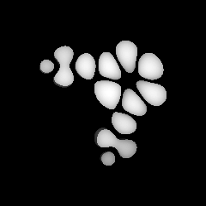
\includegraphics[width=0.45\textwidth]{homo} &
				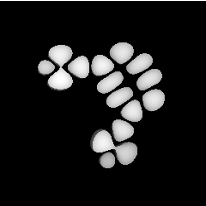
\includegraphics[width=0.45\textwidth]{lumo} \\
				\SI{-11.601}{\electronvolt} & \SI{-10.134 }{\electronvolt} \\
			\end{tabular}
		\end{minipage}
		\hfill
		%
		\begin{minipage}{0.2\textwidth} \centering
			Insert fancy Energy graph here...	
		\end{minipage}
	\end{figure}
	%%%%%%%%%%%%%%%%%%%%%%%%%%%%%%%%%%%%%%%%%%%%%%%%%%%%%%%%%%%%%%%%%%%%%%%%%%%%%%%%%%
	%%%%%%%%%%%%%%%%%%%%%%%%%%%%%%%%%%%%%%%%%%%%%%%%%%%%%%%%%%%%%%%%%%%%%%%%%%%%%%%%%%
	\begin{figure}[]
		\centering
		\subfigure[]{
			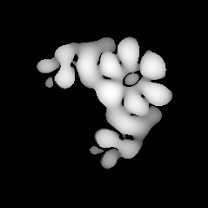
\includegraphics[width=0.2\textwidth]{int-homo-1}
			\label{fig:}
		}
		\subfigure[HOMO - 1]{
			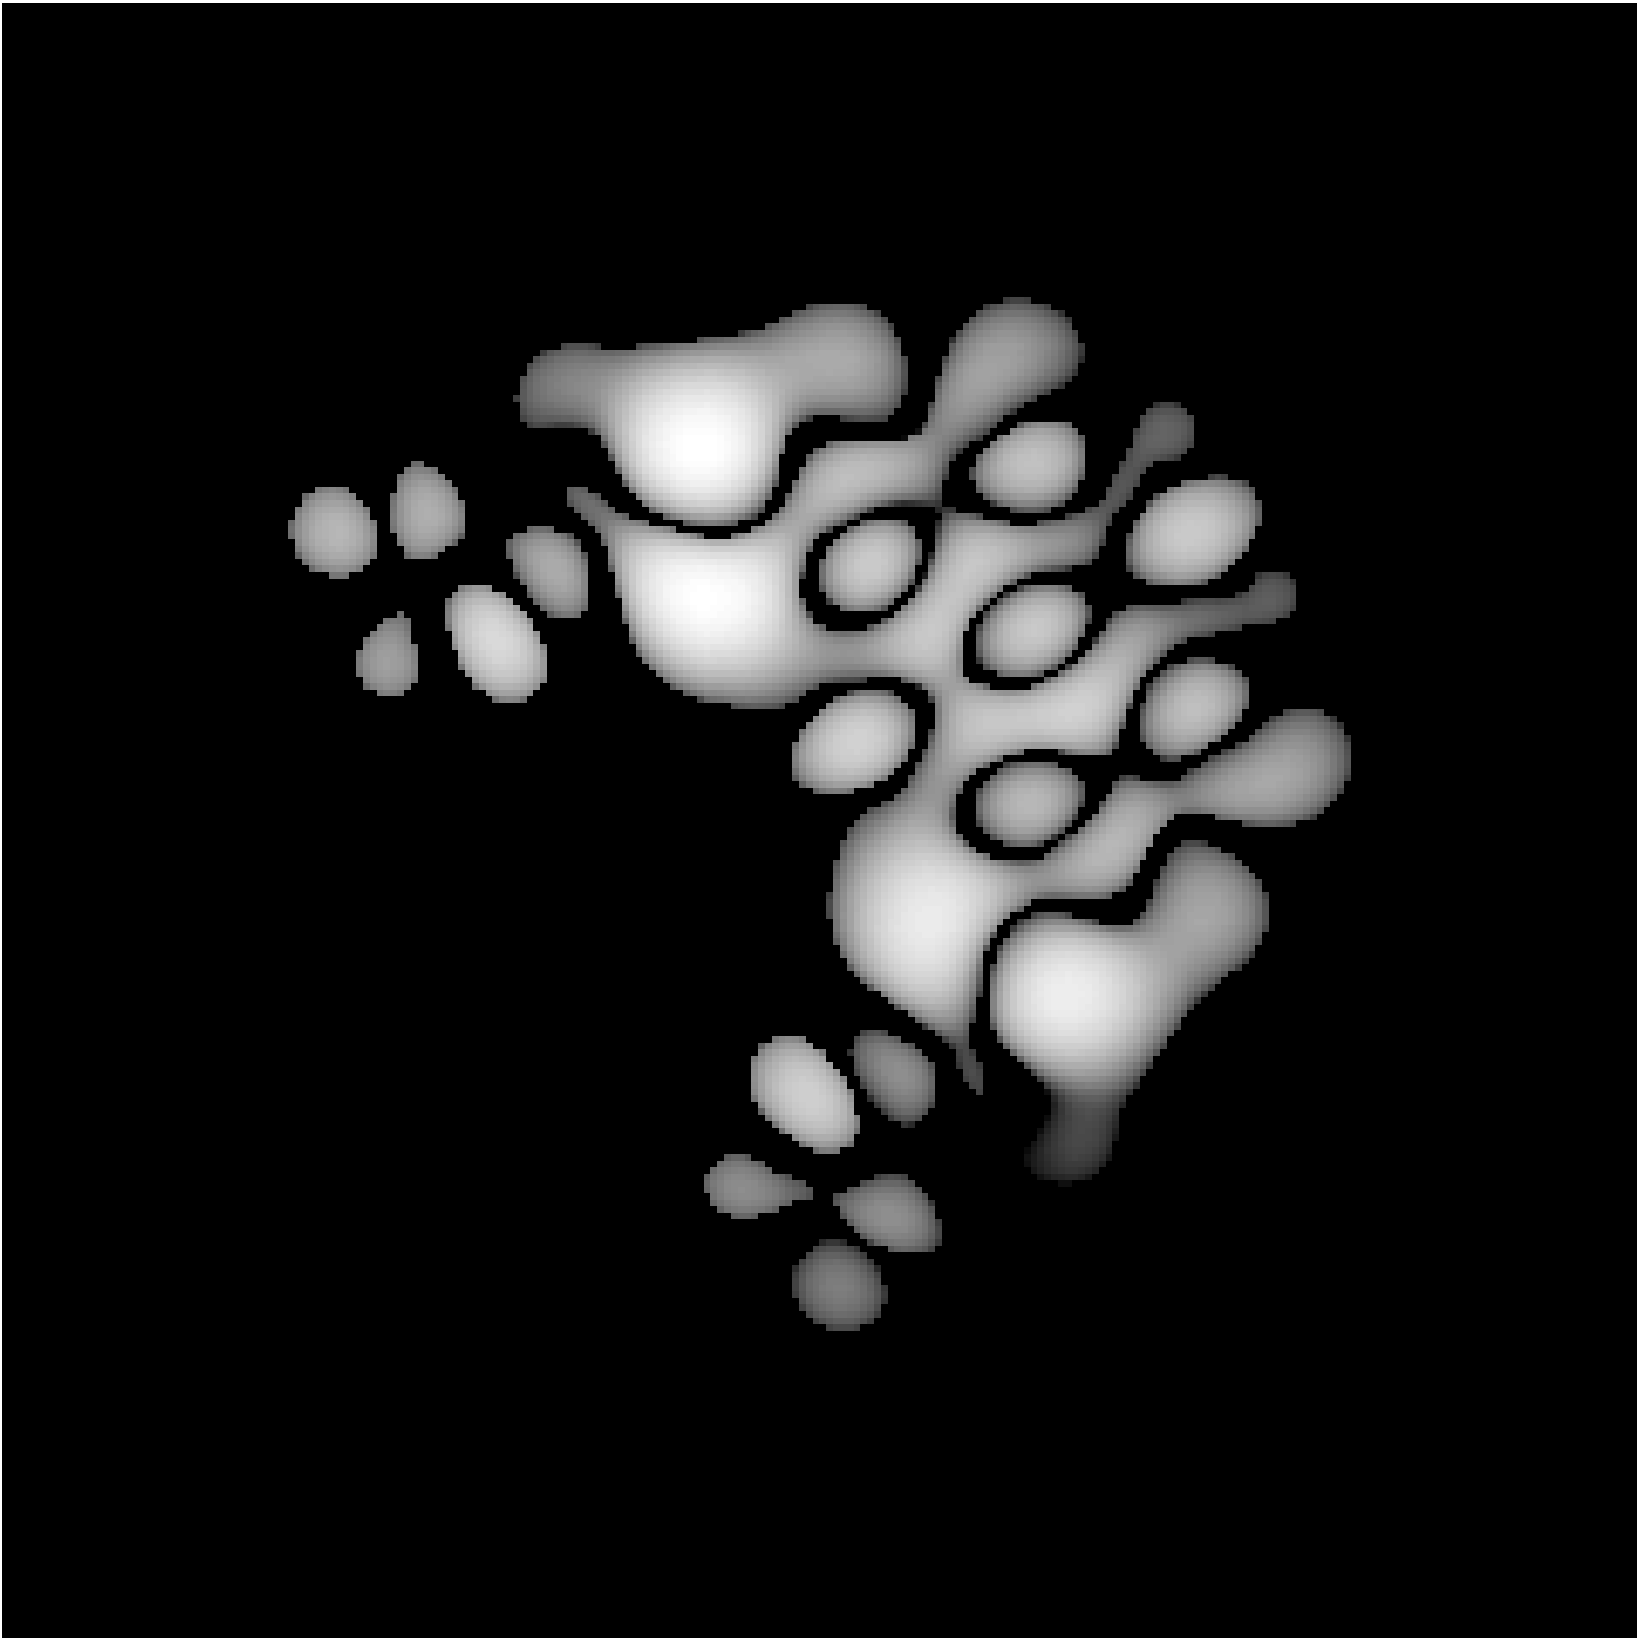
\includegraphics[width=0.2\textwidth]{homo-1}
			\label{fig:homo-1}	
		}
		\subfigure[LUMO + 1]{
			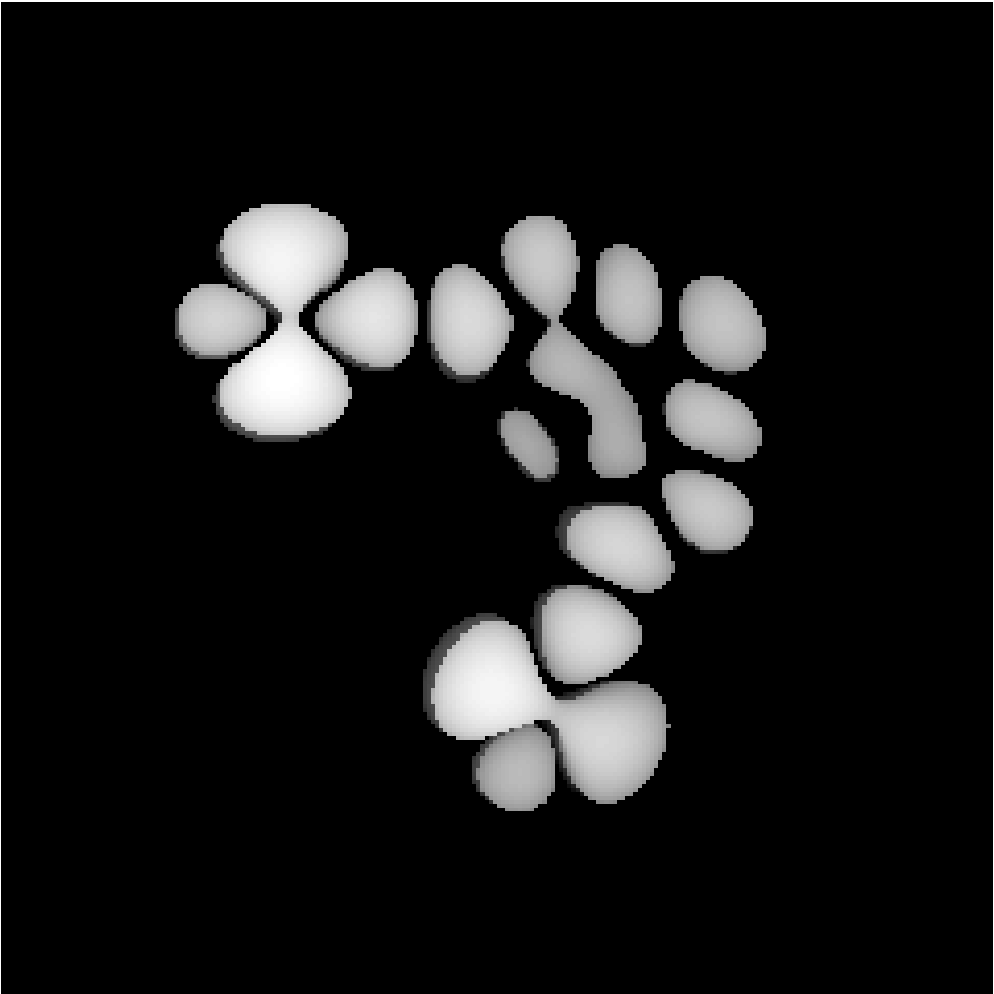
\includegraphics[width=0.2\textwidth]{lumo-1}
			\label{fig:lumo+1}	
		}
		\subfigure[]{
			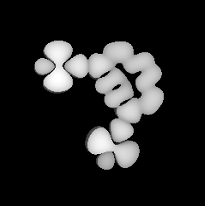
\includegraphics[width=0.2\textwidth]{int-lumo-1}
			\label{fig:}	
		}
		%%%%%%%%%%%%%%%%%%%%%%%%%%%%%%%%%%%%%%%%%
		\subfigure[]{
			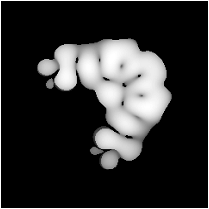
\includegraphics[width=0.2\textwidth]{int-homo-2}
			\label{fig:}
		}
		\subfigure[HOMO - 2]{
			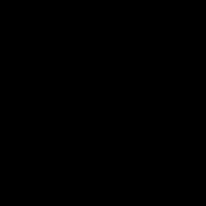
\includegraphics[width=0.2\textwidth]{homo-2}
			\label{fig:homo-2}	
		}
		\subfigure[LUMO + 2]{
			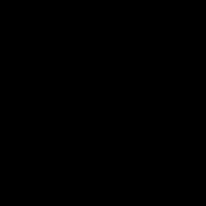
\includegraphics[width=0.2\textwidth]{lumo-2}
			\label{fig:lumo+2}	
		}
		\subfigure[]{
			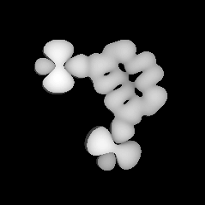
\includegraphics[width=0.2\textwidth]{int-lumo-2}
			\label{fig:}	
		}
		%%%%%%%%%%%%%%%%%%%%%%%%%%%%%%%%%%%%%%%%%
		\subfigure[]{
			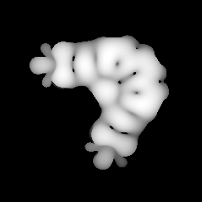
\includegraphics[width=0.2\textwidth]{int-homo-3}
			\label{fig:}
		}
		\subfigure[HOMO - 3]{
			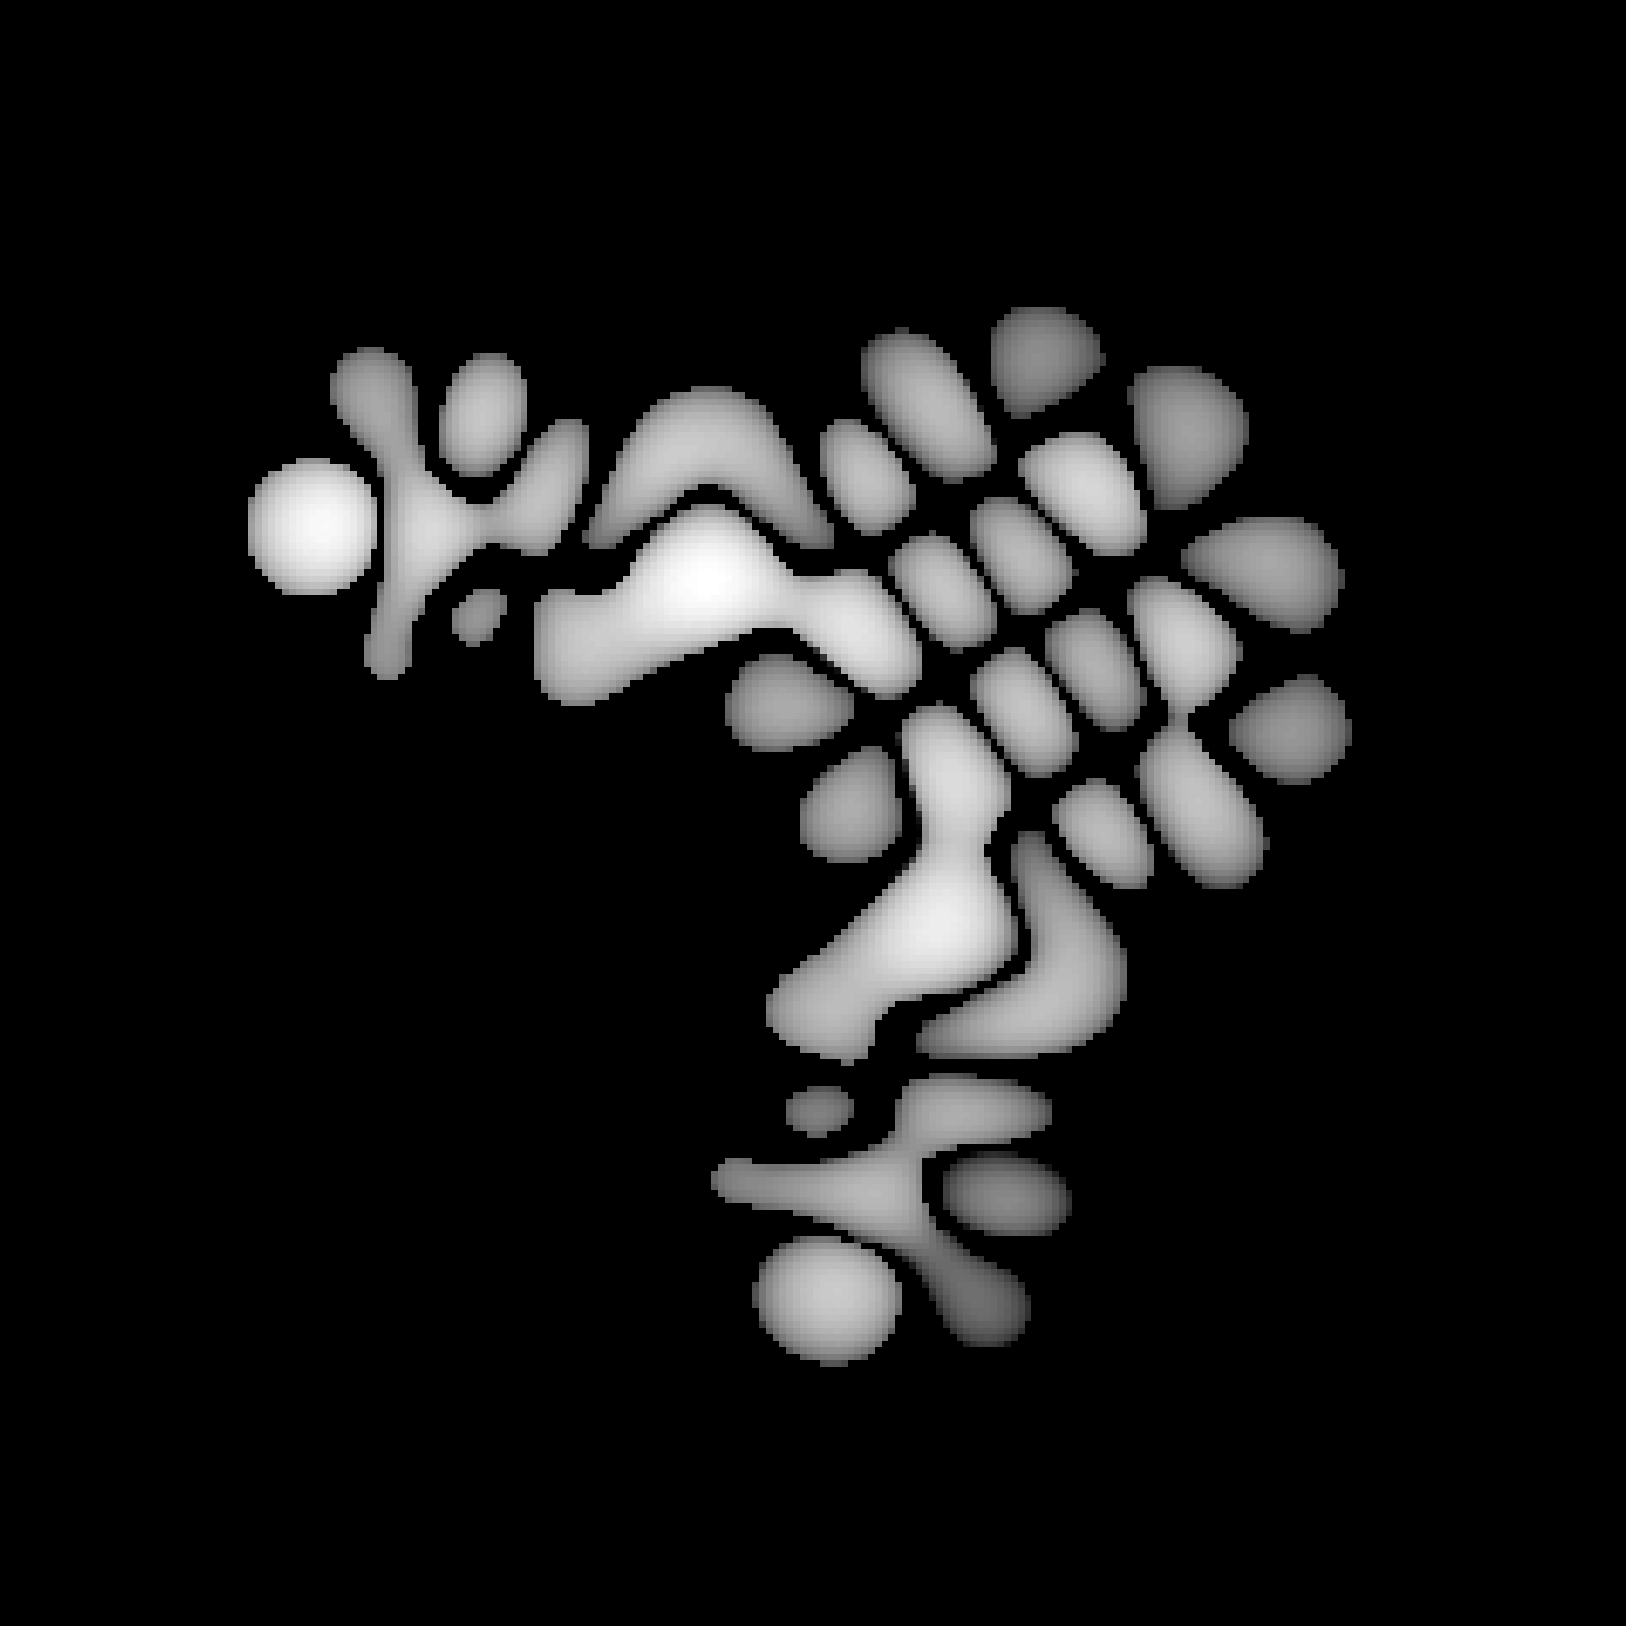
\includegraphics[width=0.2\textwidth]{homo-3}
			\label{fig:homo-3}	
		}
		\subfigure[LUMO + 3]{
			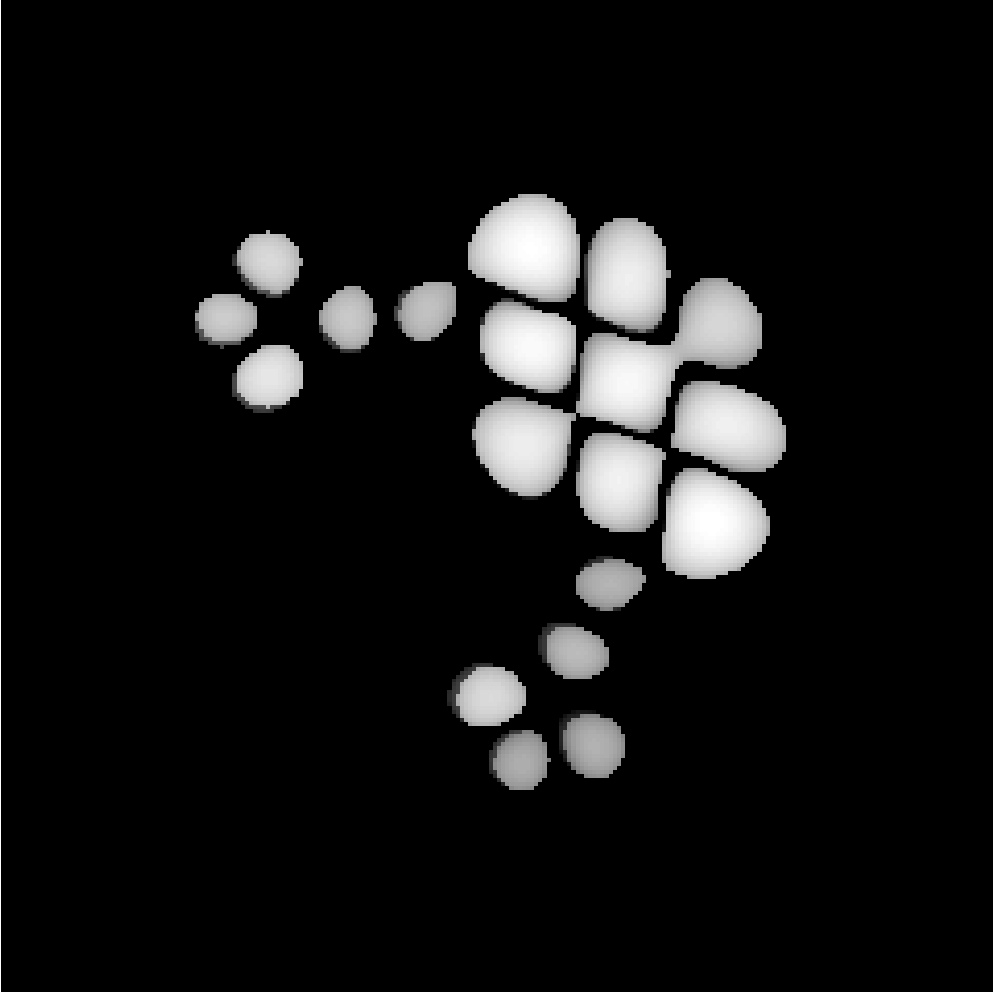
\includegraphics[width=0.2\textwidth]{lumo-3}
			\label{fig:lumo+3}	
		}
		\subfigure[]{
			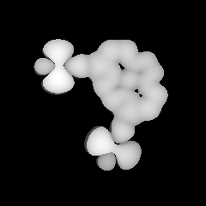
\includegraphics[width=0.2\textwidth]{int-lumo-3}
			\label{fig:}	
		}
		%%%%%%%%%%%%%%%%%%%%%%%%%%%%%%%%%%%%%%%%%
		\subfigure[]{
			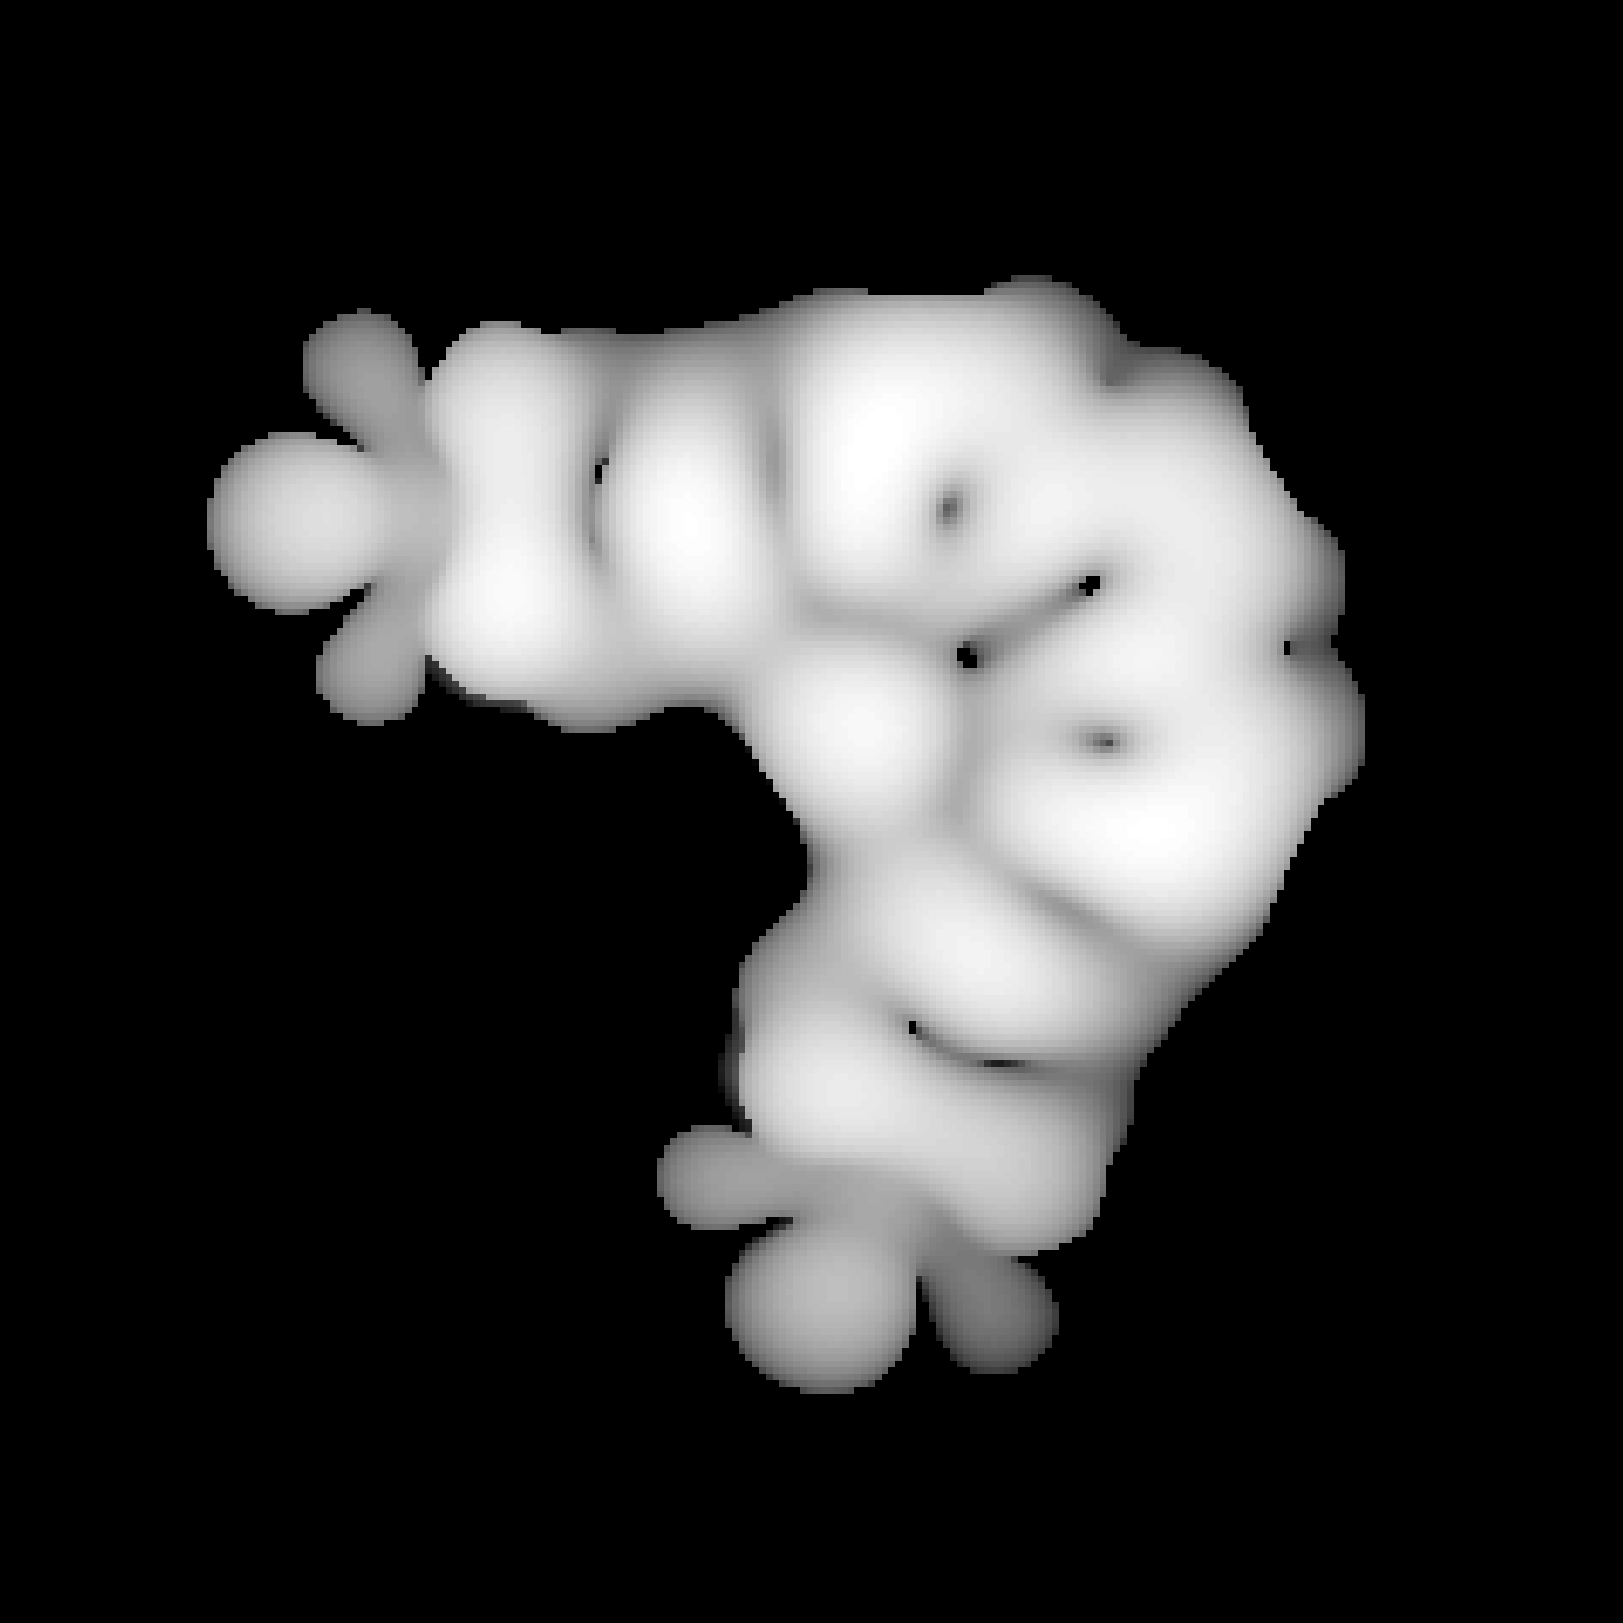
\includegraphics[width=0.2\textwidth]{int-homo-4}
			\label{fig:}
		}
		\subfigure[HOMO - 4]{
			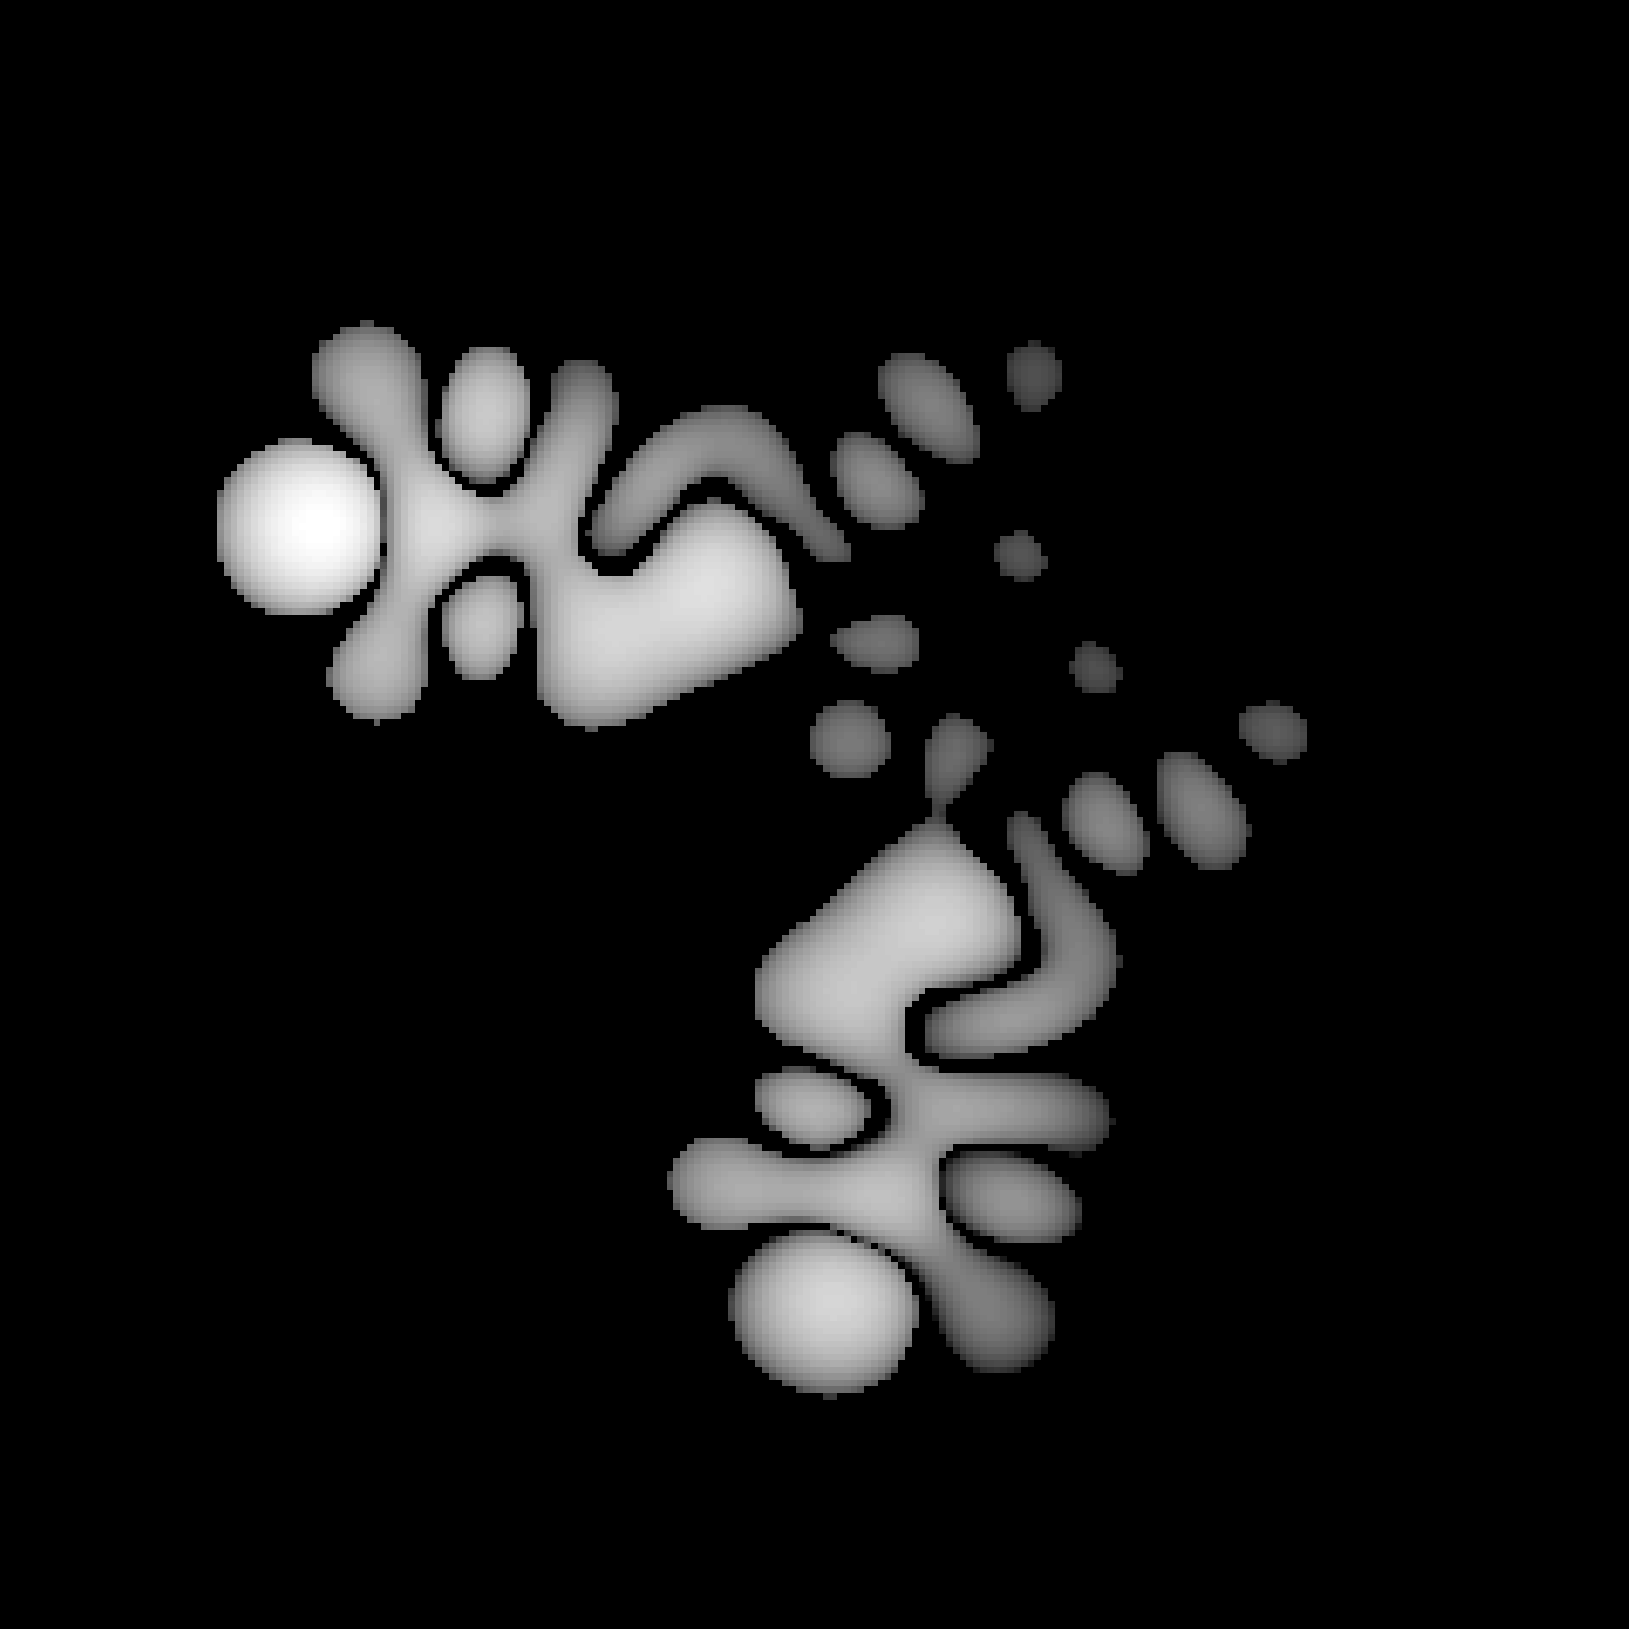
\includegraphics[width=0.2\textwidth]{homo-4}
			\label{fig:homo-4}	
		}
		\subfigure[LUMO + 4]{
			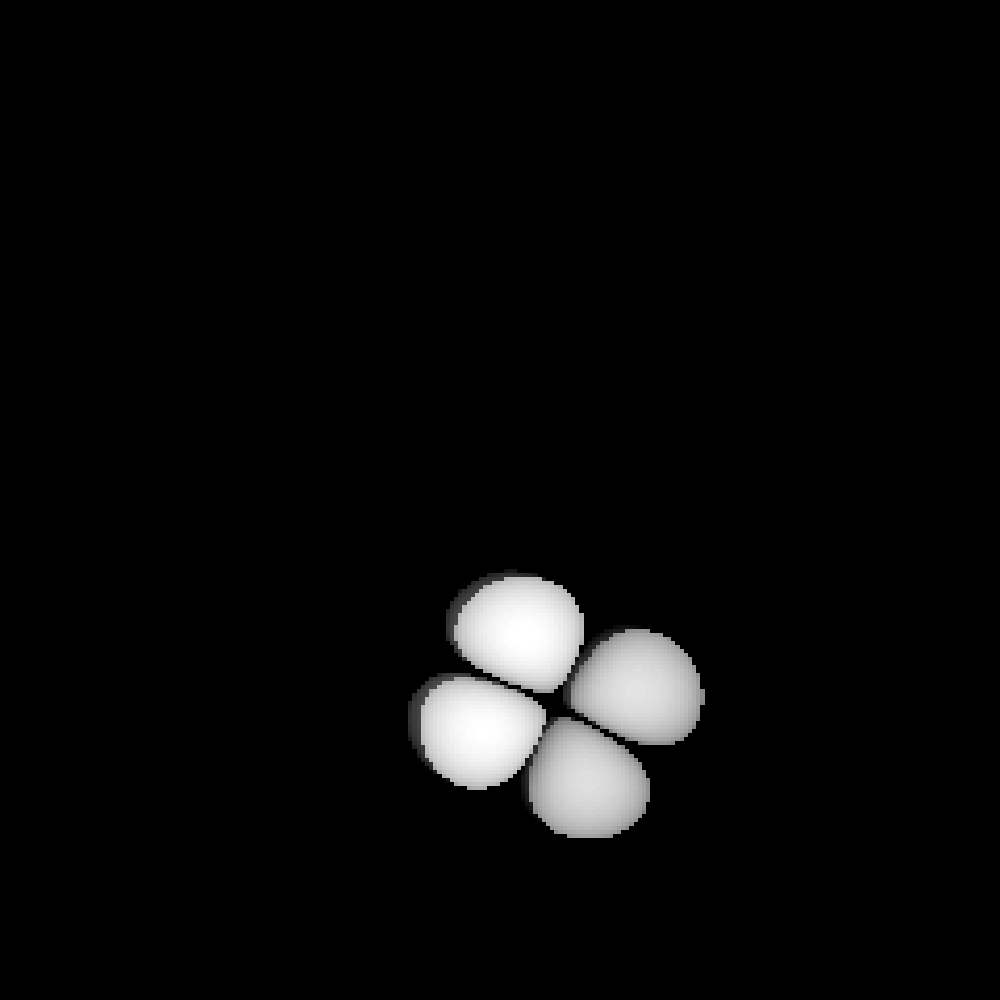
\includegraphics[width=0.2\textwidth]{lumo-4}
			\label{fig:lumo+4}	
		}
		\subfigure[]{
			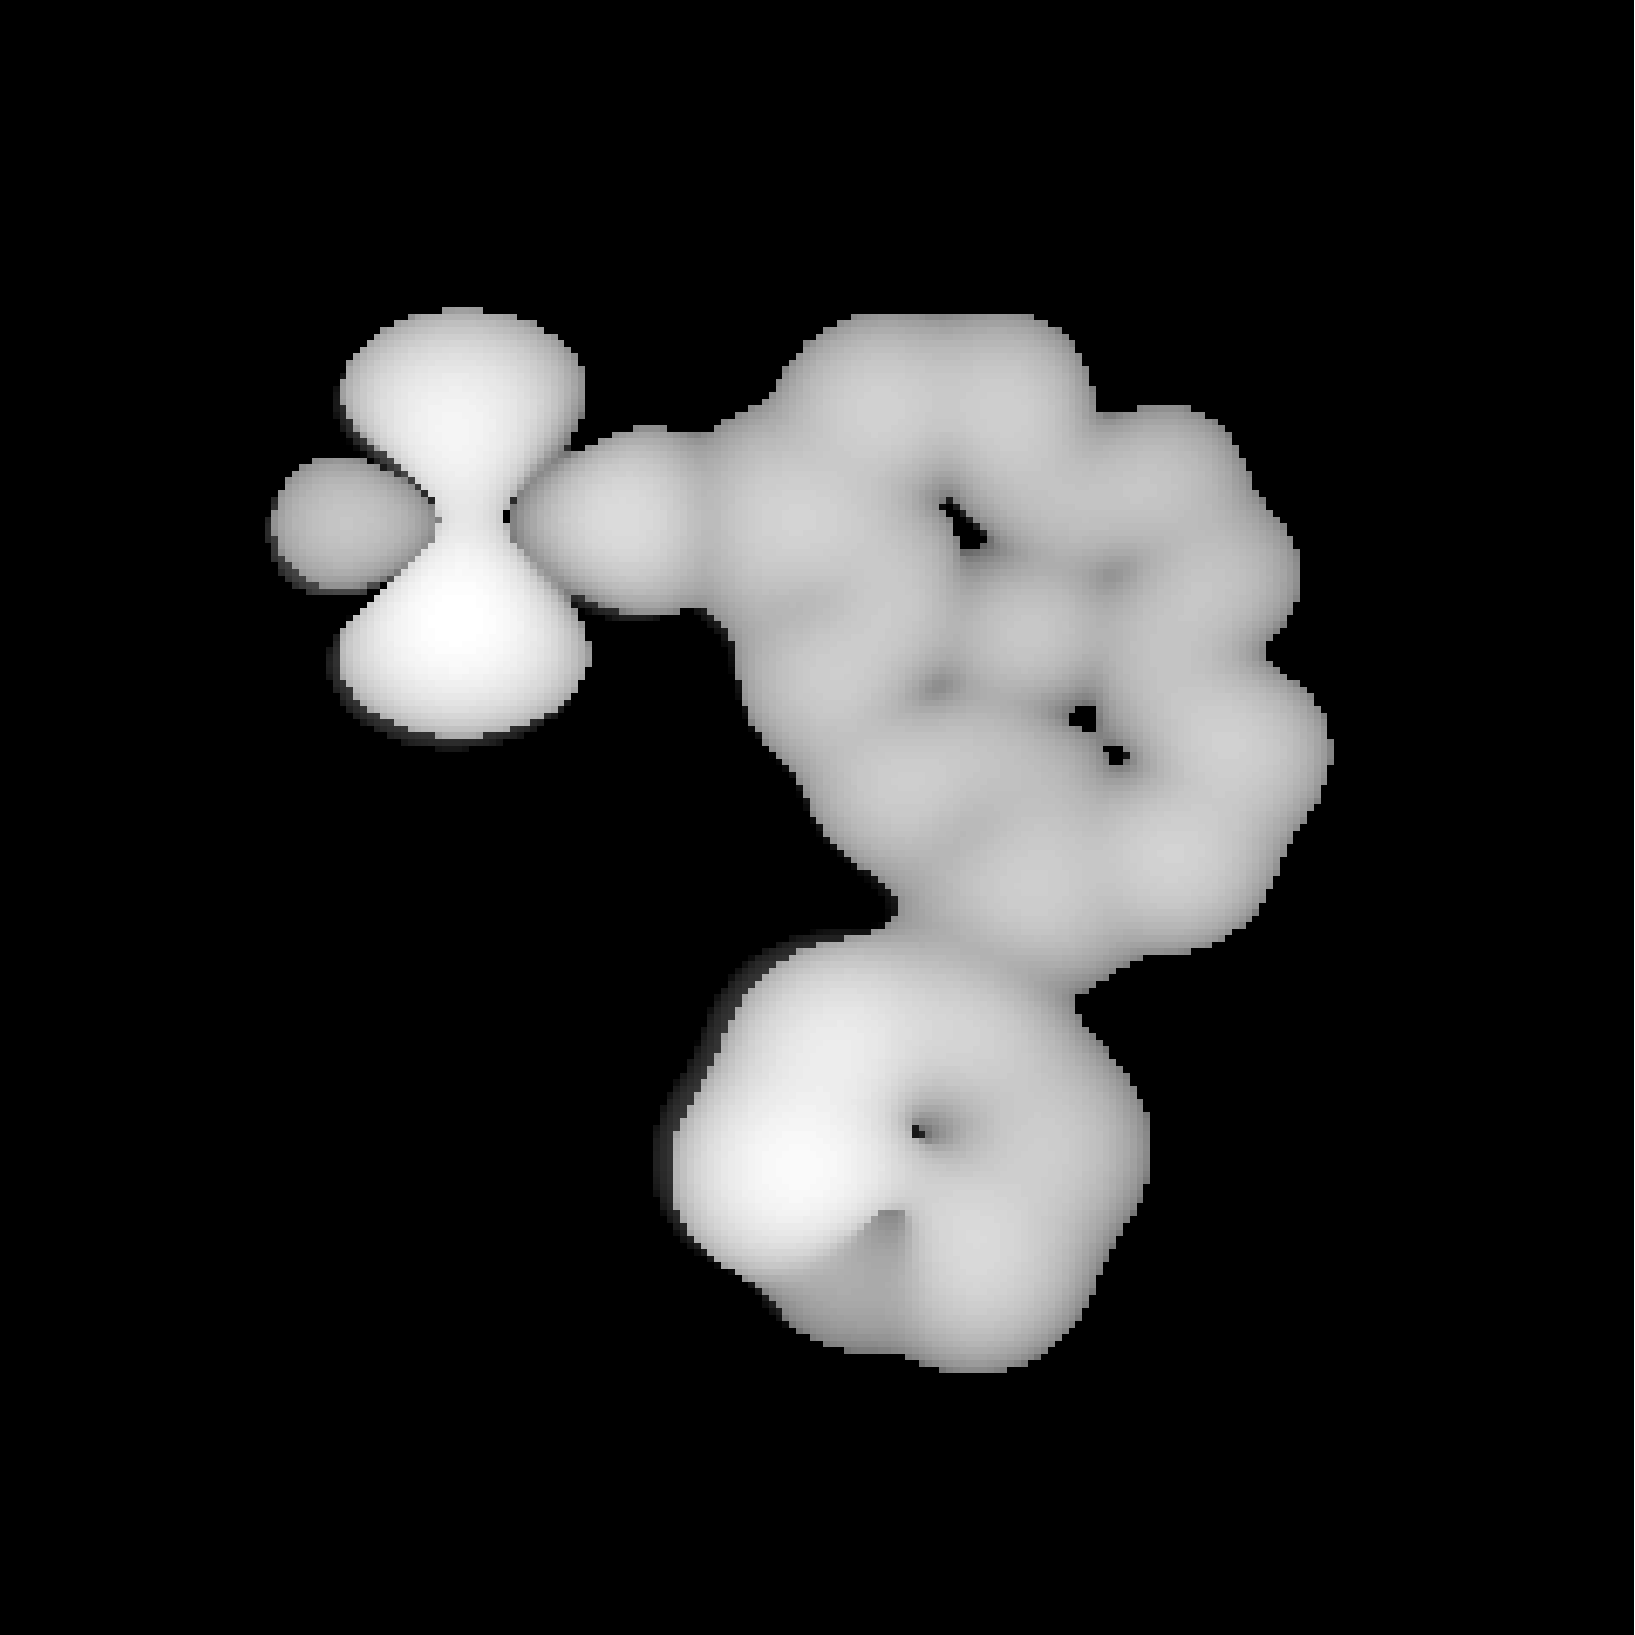
\includegraphics[width=0.2\textwidth]{int-lumo-4}
			\label{fig:}	
		}
		%%%%%%%%%%%%%%%%%%%%%%%%%%%%%%%%%%%%%%%%%
		\subfigure[]{
			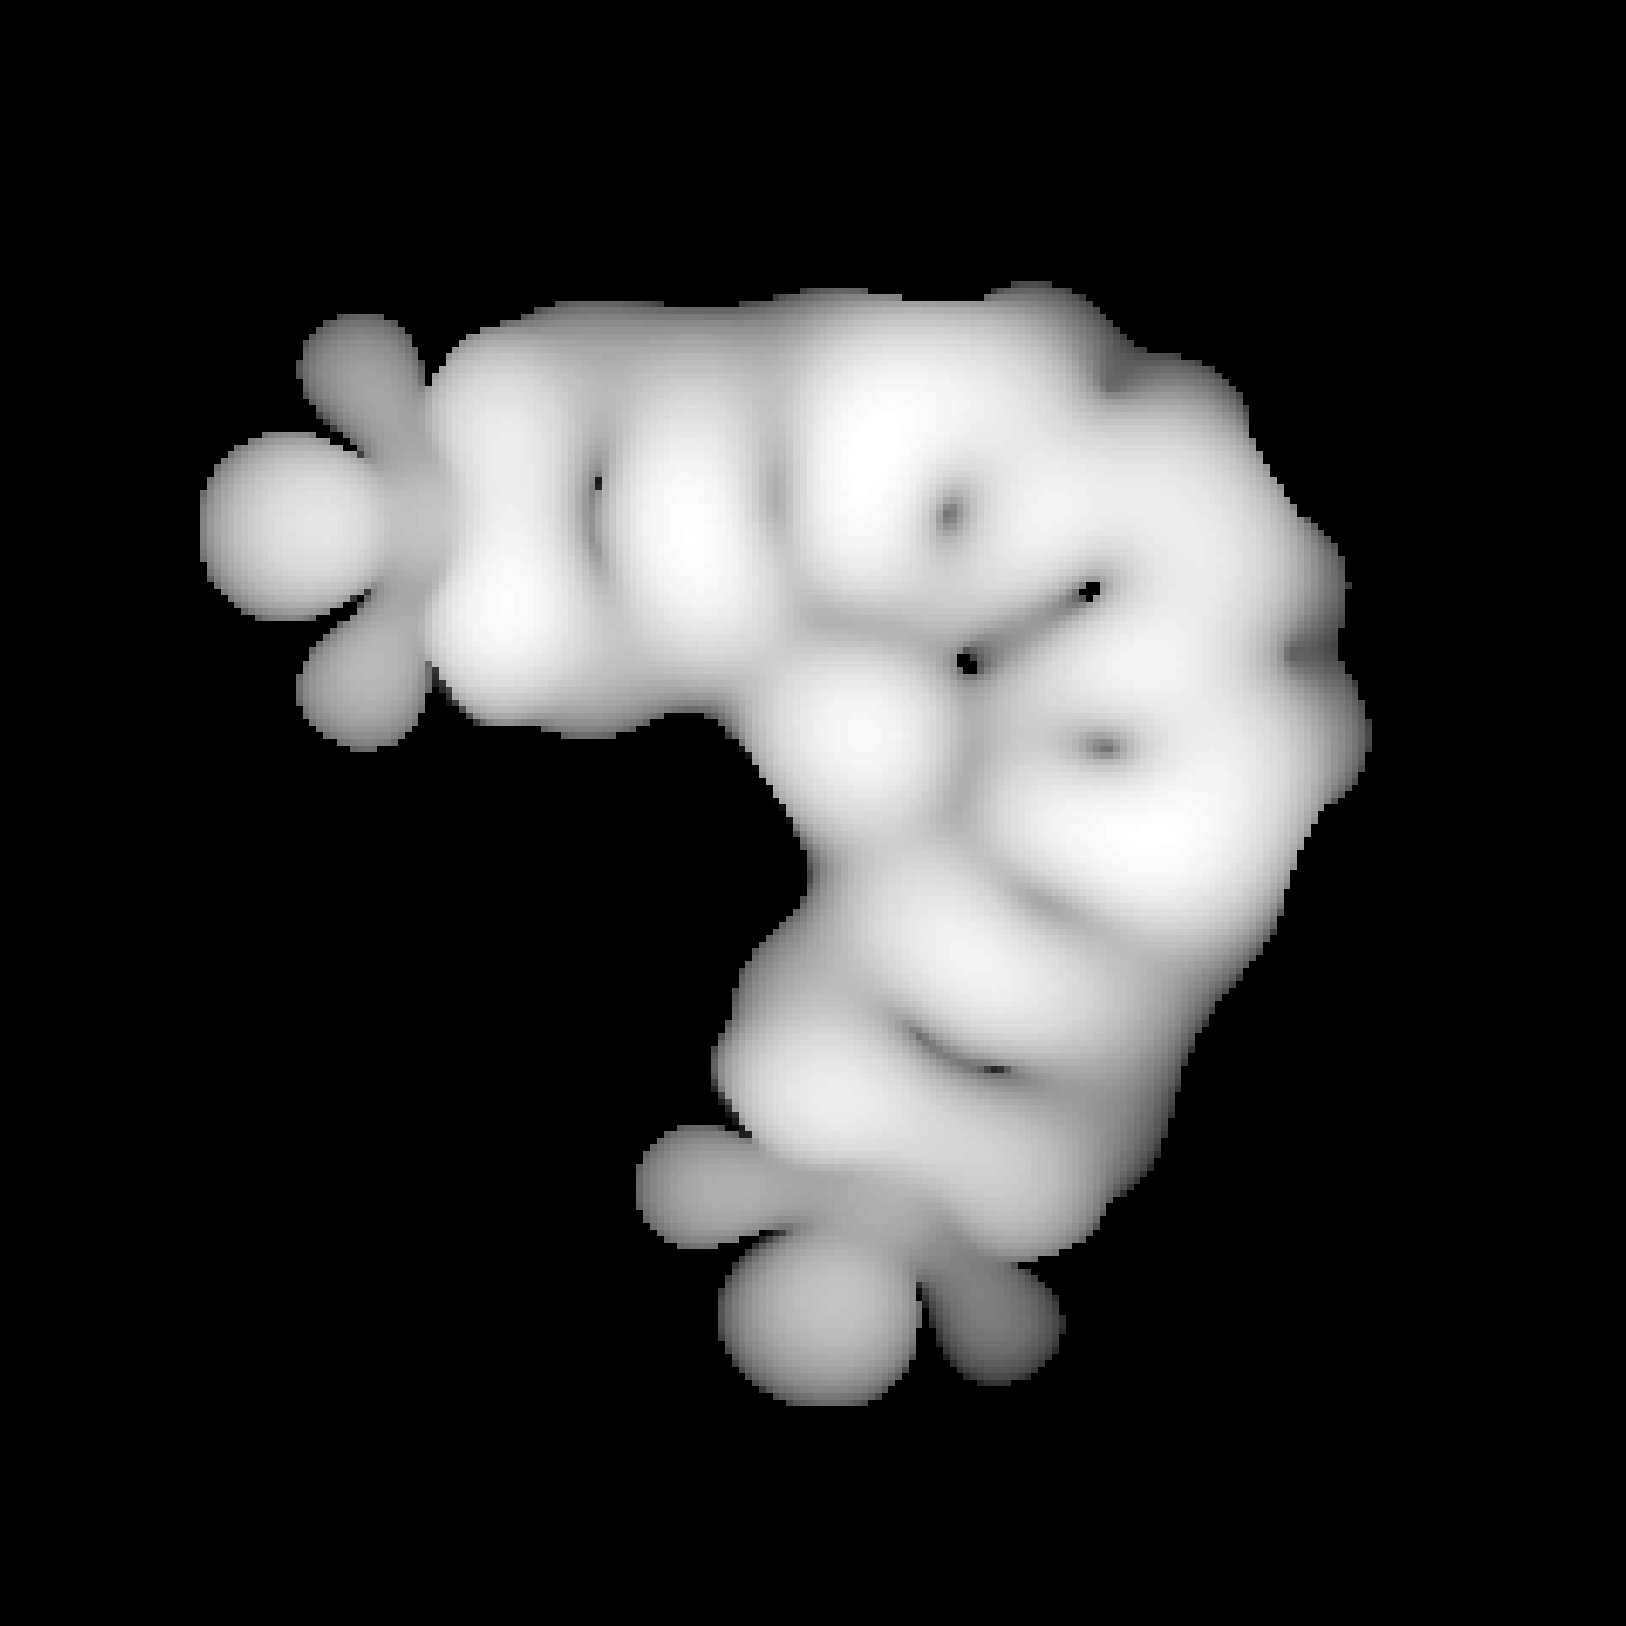
\includegraphics[width=0.2\textwidth]{int-homo-5}
			\label{fig:}
		}
		\subfigure[HOMO - 5]{
			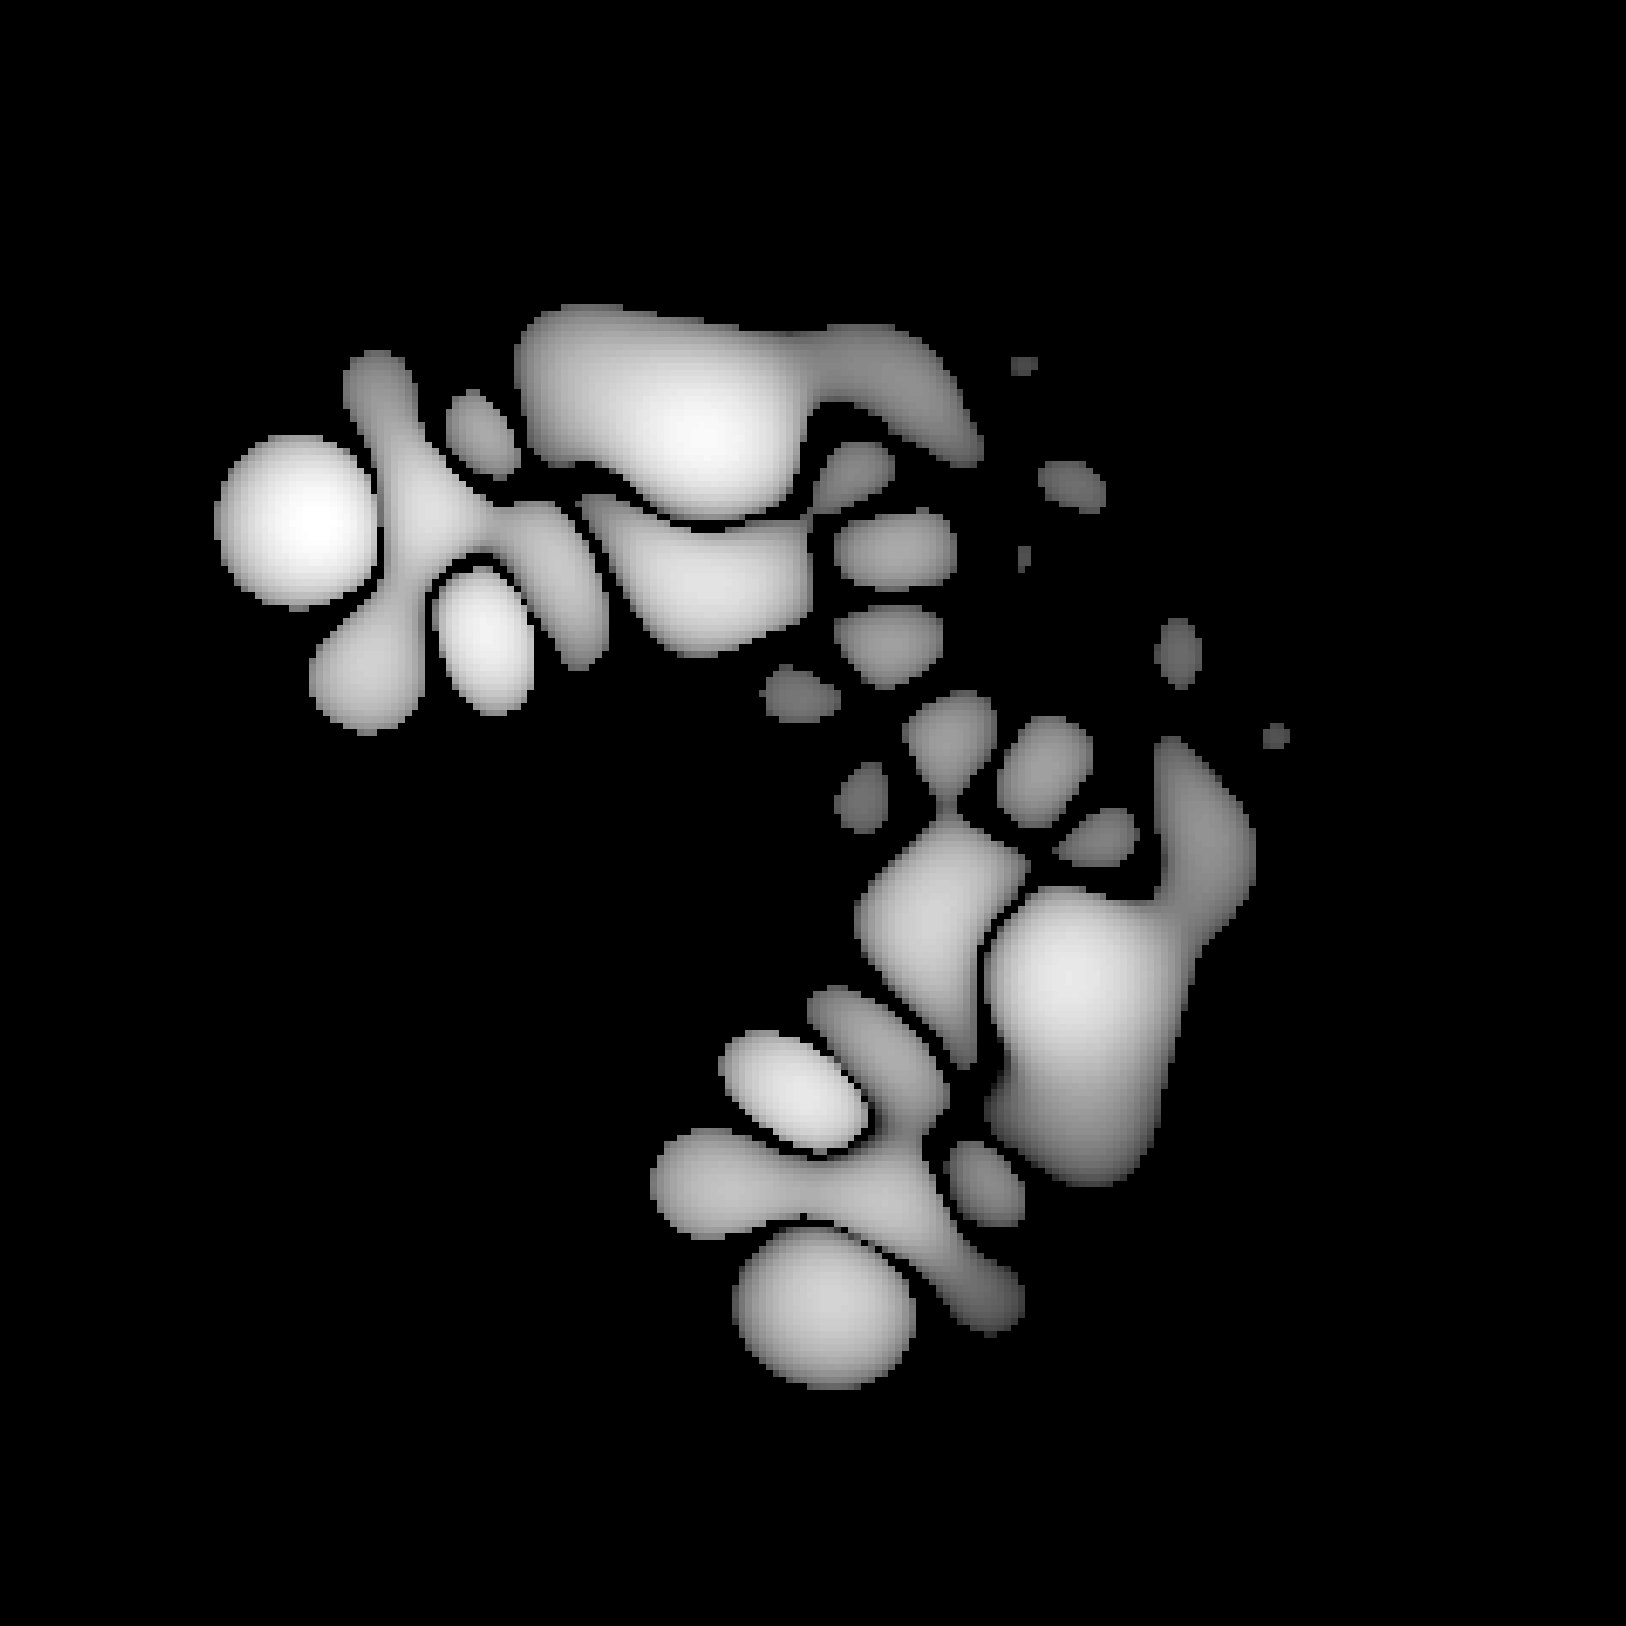
\includegraphics[width=0.2\textwidth]{homo-5}
			\label{fig:homo-5}	
		}
		\subfigure[LUMO + 5]{
			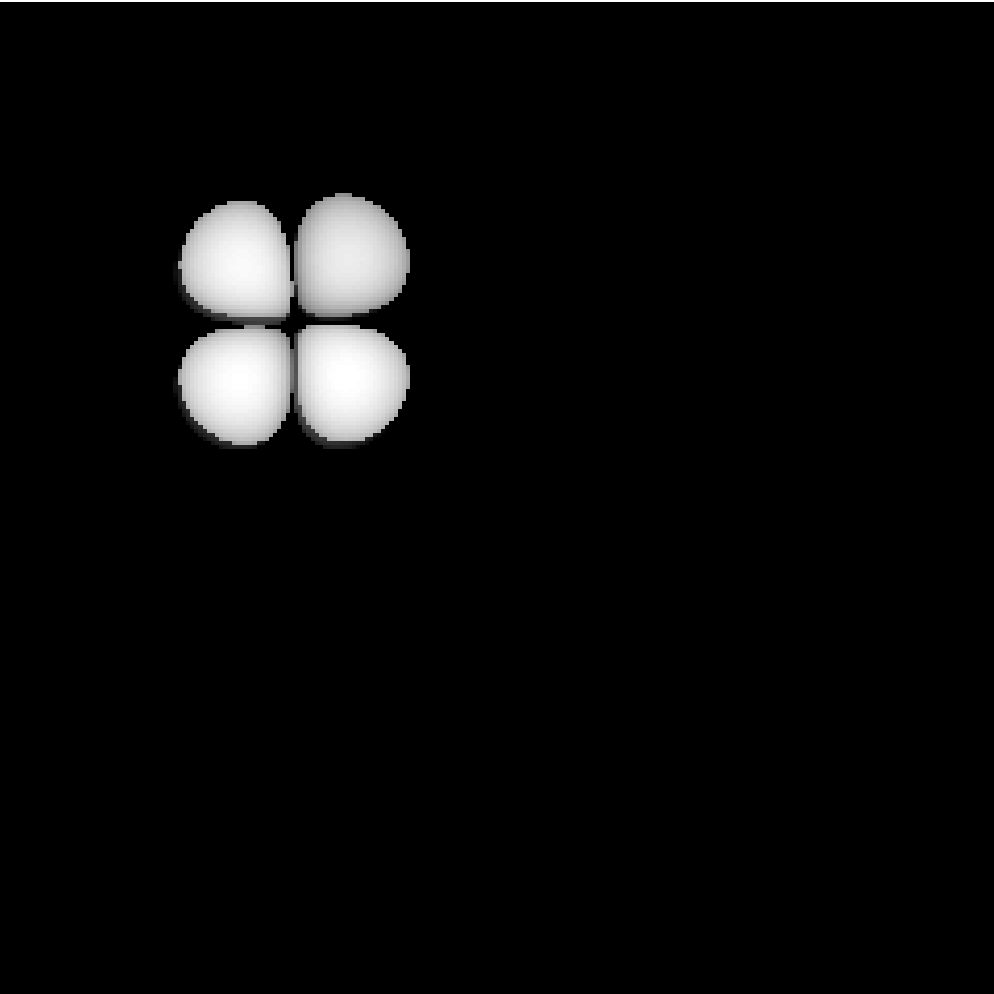
\includegraphics[width=0.2\textwidth]{lumo-5}
			\label{fig:lumo+5}	
		}
		\subfigure[]{
			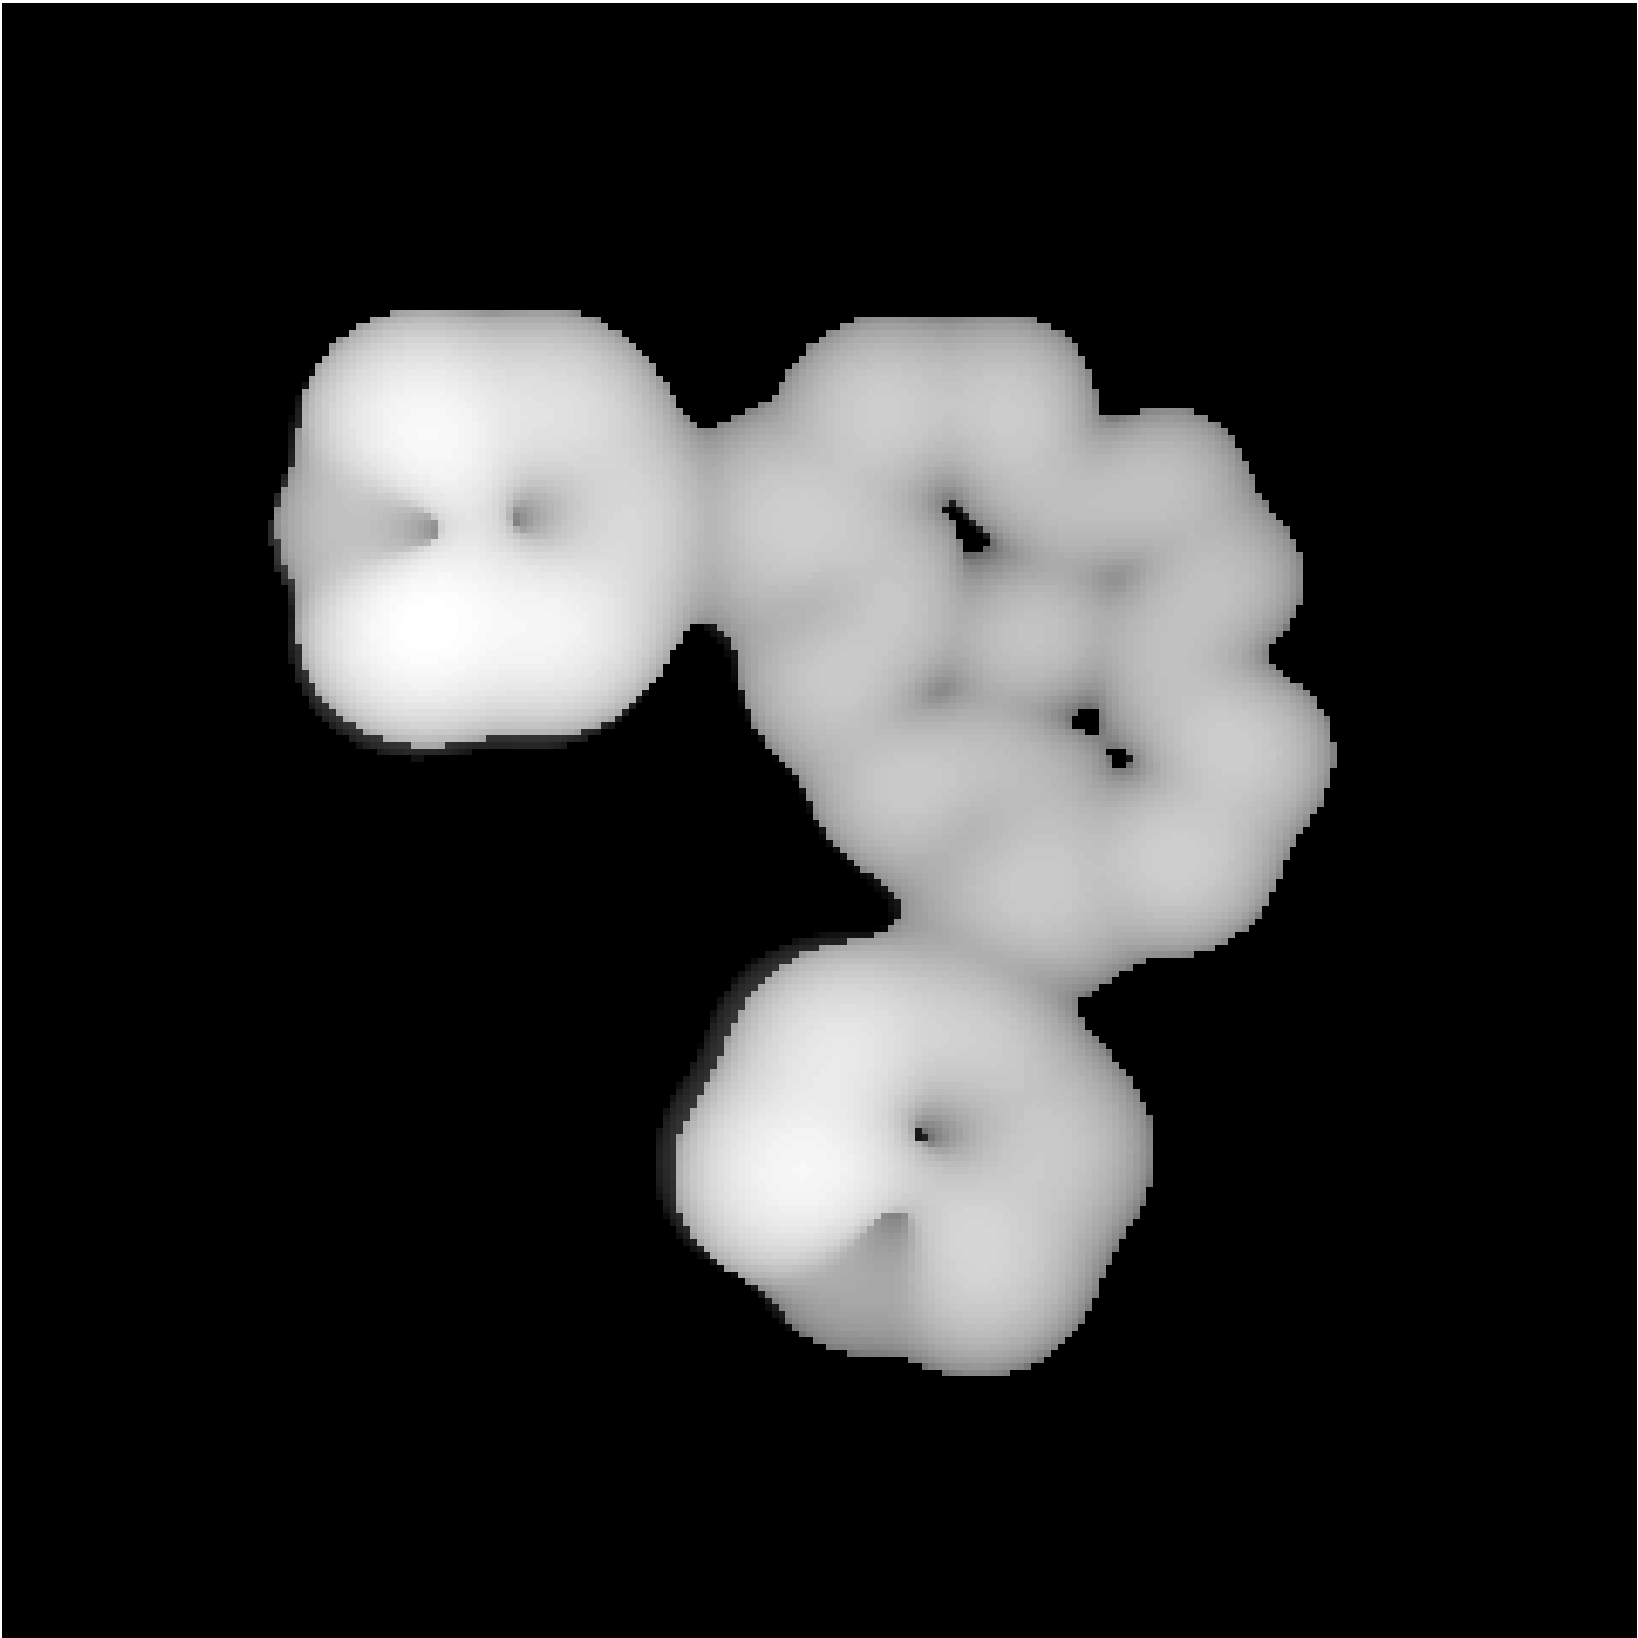
\includegraphics[width=0.2\textwidth]{int-lumo-5}
			\label{fig:}	
		}
		\caption{EHT calculated molecular orbitals. HOMO and LUMO states together with five neighboring states (shown in the same column). Inner two columns show HOMO \& LUMO states. Outer columns show integration of states as STM image estimation if all states to $E_F$ were contributing equally.}
		\label{fig:}
	\end{figure}
	\vfill
	\restoregeometry